\documentclass[11pt,letterpaper]{article}

\usepackage[margin=0.85in,headheight=16pt]{geometry}
\usepackage[T1]{fontenc}
\usepackage[utf8]{inputenc}
\usepackage{lmodern,microtype}
\usepackage[svgnames]{xcolor}
\usepackage{booktabs,longtable,tabularx,array}
\usepackage{enumitem,hyperref,bookmark,fancyhdr,lastpage,xurl}
\usepackage{listings,tcolorbox,graphicx}
\usepackage{titlesec,tikz}
\usetikzlibrary{positioning,arrows.meta,shapes.geometric}
\definecolor{navy}{HTML}{142E4B}
\definecolor{teal}{HTML}{087D7A}
\definecolor{light}{HTML}{F3F7FA}
\definecolor{codebg}{HTML}{F5F7FA}
\hypersetup{colorlinks=true,urlcolor=teal,linkcolor=navy,pdfauthor={Software Build Engineering},pdfsubject={CMake and WebAssembly platform architecture}}
\titleformat{\section}{\Large\bfseries\color{navy}}{\thesection}{0.7em}{}
\titleformat{\subsection}{\large\bfseries\color{teal}}{\thesubsection}{0.7em}{}
\setlength{\emergencystretch}{2em}
\setlist[itemize]{leftmargin=*,itemsep=2pt,topsep=4pt}
\setlist[enumerate]{leftmargin=*,itemsep=3pt,topsep=4pt}
\lstdefinestyle{code}{basicstyle=\ttfamily\footnotesize,backgroundcolor=\color{codebg},breaklines=true,breakatwhitespace=false,columns=fullflexible,frame=single,rulecolor=\color{gray!25},showstringspaces=false,tabsize=2,keepspaces=true,postbreak=\mbox{\textcolor{red}{$\hookrightarrow$}\space}}
\lstset{style=code}
\tcbset{colback=light,colframe=teal!65!black,arc=1mm,boxrule=0.7pt,left=8pt,right=8pt,top=6pt,bottom=6pt}
\newtcolorbox{principle}[1]{title={#1},fonttitle=\bfseries\small}
\newcommand{\DocHeader}[3]{\title{\sffamily\color{navy}\bfseries #1\\[9pt]\large\normalfont\color{teal} #2}\author{Cross-Platform Build Engineering | Reference Edition}\date{Version #3 \quad--\quad 17 October 2026}}
\pagestyle{fancy}\fancyhf{}\lhead{\small CMake / WebAssembly Engineering}\rhead{\small\color{teal}\leftmark}\cfoot{\small Page \thepage\ of \pageref{LastPage}}
\renewcommand{\headrulewidth}{0.4pt}
\newcommand{\frontmatterdoc}{\maketitle\vspace{2mm}\begin{principle}{Document status}\textbf{Classification:} Engineering guidance and tested reference patterns, not a normative specification. Version pins reflect the specified reference baseline. Production use requires testing against the target SDK, runtime, threat model, and dependency set.\end{principle}\tableofcontents\clearpage}
\newcommand{\accept}[1]{\par\noindent\textbf{Acceptance criterion:} #1\par}
\newcommand{\sourceurl}[1]{\par\noindent\footnotesize\url{#1}\normalsize}

% Integration note (2026-10-18): five suite volumes reference a companion
% ../reference/ source tree (CMakeLists.txt, CMakePresets.json, scripts,
% tests, browser/web clients) that was not part of the documentation upload
% batches and could not be recovered. \lstinputlisting falls back to a
% clearly marked notice when a referenced file is absent so the volumes stay
% buildable; restoring the files next to the suite re-enables the listings.
\makeatletter
\let\cmakewasm@lstinputlisting\lstinputlisting
\renewcommand{\lstinputlisting}[2][]{%
  \IfFileExists{#2}{\cmakewasm@lstinputlisting[#1]{#2}}{%
    \begin{tcolorbox}[colback=light,colframe=navy!60]\small
      \textbf{Referenced listing not included in this repository:}
      \texttt{\detokenize{#2}}. The companion reference tree was not part of
      the documentation upload; the surrounding guidance is unaffected.
    \end{tcolorbox}}}
\makeatother

\DocHeader{Reference Architecture and Decisions}{SUBReference Architecture and Decisions}{1.0}
\begin{document}
\frontmatterdoc
\section{Engineering problem and decisions}
A CMake project selects a compiler, linker, system root, and platform model when it is configured. Compiling the same source on three platforms does \emph{not} produce three interchangeable executables. In particular, Emscripten's generated JavaScript runtime is an application host, while WASI relies on a separately provisioned capability-based host. Native executables use the platform OS and native ABI directly.

\begin{principle}{Architecture thesis}
Keep data transformations and portable algorithms in a target named \texttt{portable\_core}. Connect them to three separate entrypoints: \texttt{portable\_cli} (native and WASI), \texttt{portable\_browser} (Emscripten only), and dedicated CTest binaries. Platform-specific compile definitions and link flags belong to their adapter targets, never to an unqualified global build setting.
\end{principle}

\section{Logical and deployment architecture}
\begin{center}\small
\noindent\begin{tabularx}{\linewidth}{>{\bfseries}p{0.19\linewidth}X X}
\toprule
Zone & Responsibilities & Deployable artifact \\
\midrule
Domain core & Algorithms, validation, portable data contracts, deterministic behavior & Static library linked separately for each toolchain \\
Browser adapter & C ABI exports, JS wrapper, buffer ownership, asynchronous module initialization & ES module, \texttt{.wasm}, web assets \\
WASI adapter & Command entrypoint, host capability requests, guest ABI contracts & WASI \texttt{.wasm} module or component \\
Native adapter & OS integration, process lifecycle, debugging interfaces & Native executable and optional shared library \\
Validation plane & Native CTest, Node ABI smoke tests, browser E2E, Wasmtime CTest, binary checks & Logs, checksums, provenance metadata \\
\bottomrule
\end{tabularx}
\end{center}
The dependency direction is \textbf{adapters $\rightarrow$ core}; reverse imports are forbidden. Host APIs are replaced by a port interface and provided through explicit dependency injection. Host policy, not a WASM extension, determines how much filesystem/network/process authority a module receives.


\subsection{Deployment view (not to scale)}
\begin{center}
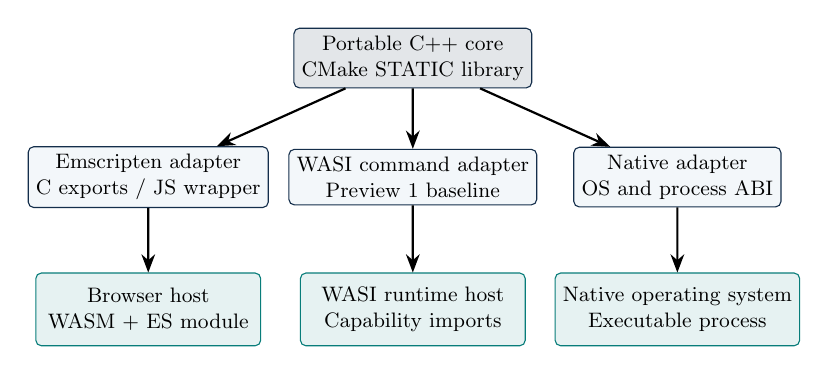
\begin{tikzpicture}[>=Stealth,scale=0.84,transform shape,rounded corners=2pt,
 every node/.style={font=\small,align=center},box/.style={draw=navy,fill=light,minimum width=3.1cm,minimum height=0.8cm},host/.style={draw=teal,fill=teal!10,minimum width=3.4cm,minimum height=1.1cm}]
\node[box,fill=navy!12] (core) at (0,2.2) {Portable C++ core\\CMake STATIC library};
\node[box] (browser) at (-4.0,0.4) {Emscripten adapter\\C exports / JS wrapper};
\node[box] (wasi) at (0,0.4) {WASI command adapter\\Preview 1 baseline};
\node[box] (native) at (4.0,0.4) {Native adapter\\OS and process ABI};
\node[host] (web) at (-4.0,-1.6) {Browser host\\WASM + ES module};
\node[host] (wasmtime) at (0,-1.6) {WASI runtime host\\Capability imports};
\node[host] (os) at (4.0,-1.6) {Native operating system\\Executable process};
\draw[->,thick] (core) -- (browser); \draw[->,thick] (core) -- (wasi); \draw[->,thick] (core) -- (native);
\draw[->,thick] (browser) -- (web); \draw[->,thick] (wasi) -- (wasmtime); \draw[->,thick] (native) -- (os);
\end{tikzpicture}
\end{center}
\noindent\emph{Arrows show build/deployment flow; source dependencies point from adapters to the core.}

\section{Architecture decision record register}
Each ADR documents status, context, decision, alternatives, consequences, and measurable validation. The following register defines the baseline decisions.
\begin{longtable}{p{0.13\linewidth}p{0.26\linewidth}p{0.53\linewidth}}
\toprule ID & Decision & Rationale and evidence required \\ \midrule \endhead
ADR-001 & One portable core & Prevent host SDK imports from contaminating domain code; compile it in all three variants. \\
ADR-002 & Distinct build directories & Toolchain identity is cached by CMake; no in-place native-to-WASM transition. \\
ADR-003 & Browser: C ABI + typed arrays & Predictable binary byte contract; leave Embind optional for richer objects. Test invalid lengths, memory growth, and lifetime. \\
ADR-004 & WASI: Preview 1 command baseline & Minimum viable portable CLI artifact and Wasmtime test. Do not call it a Preview 2 component. \\
ADR-005 & Preview 2 components separate & WIT contracts, component-aware tooling, and host compatibility tests precede promotion. \\
ADR-006 & Native reference oracle & Native unit tests and sanitizers detect undefined behavior before cross-target integration. \\
ADR-007 & Locked toolchain manifest & Record CMake, Emscripten, WASI SDK, runtime, dependencies, action revisions, and artifact digests. \\
ADR-008 & CI profile isolation & Independent configure/build/test jobs; test cross-target parity and publish only complete bundles. \\
ADR-009 & Provenance and verification & Build attestation ties subject digest to trusted workflow; hashes alone do not authenticate publisher. \\
ADR-010 & Least authority at runtime & Restrict exported browser APIs, enforce web security headers, and grant minimal WASI host resources. \\
\bottomrule
\end{longtable}

\section{Decision matrix and tradeoffs}
\noindent\begin{tabularx}{\linewidth}{p{0.22\linewidth}XXX}
\toprule Constraint & Browser & WASI & Native \\ \midrule
UI integration & Strong JS/DOM host & External host adapter & OS/UI framework \\
Startup model & Async instantiate & Runtime instantiate & Process start \\
Host access & Web origin and JS APIs & WASI grants/imports & OS user privileges \\
Debugging & Browser devtools & Guest + host diagnostics & OS debugger/sanitizers \\
Threads & Browser isolation prerequisites & Target/runtime-specific & OS threads \\
Distribution & Web CDN/static asset pair & Versioned module/component & OS/architecture package \\
\bottomrule
\end{tabularx}

\section{Nonfunctional architecture requirements}
\begin{enumerate}
\item Performance: publish throughput, p95 cold-start, and binary-size budgets for each profile; do not compare unlike initialization models.
\item Portability: shared tests must return identical results for fixed byte vectors across all supported targets.
\item Memory safety: bounded inputs, checked allocations, no retained typed-array view across growth, no double release.
\item Release integrity: artifact inventory reconciles to the build manifest, checksum verification, and authenticated attestation.
\item Operability: startup diagnostics identify runtime and SDK versions; host authority is declared before deployment.
\end{enumerate}
\accept{A reviewer can trace every host-specific API and toolchain flag to an adapter target and an ADR.}

\section{Source baseline}
\sourceurl{https://emscripten.org/docs/compiling/Building-Projects.html}
\sourceurl{https://github.com/WebAssembly/wasi-sdk}
\sourceurl{https://github.com/bytecodealliance/wasmtime}
\end{document}
